% REV00 Tue 04 May 2021 13:55:16 WIB
% START Tue 04 May 2021 13:55:16 WIB

\chapter{XXX}

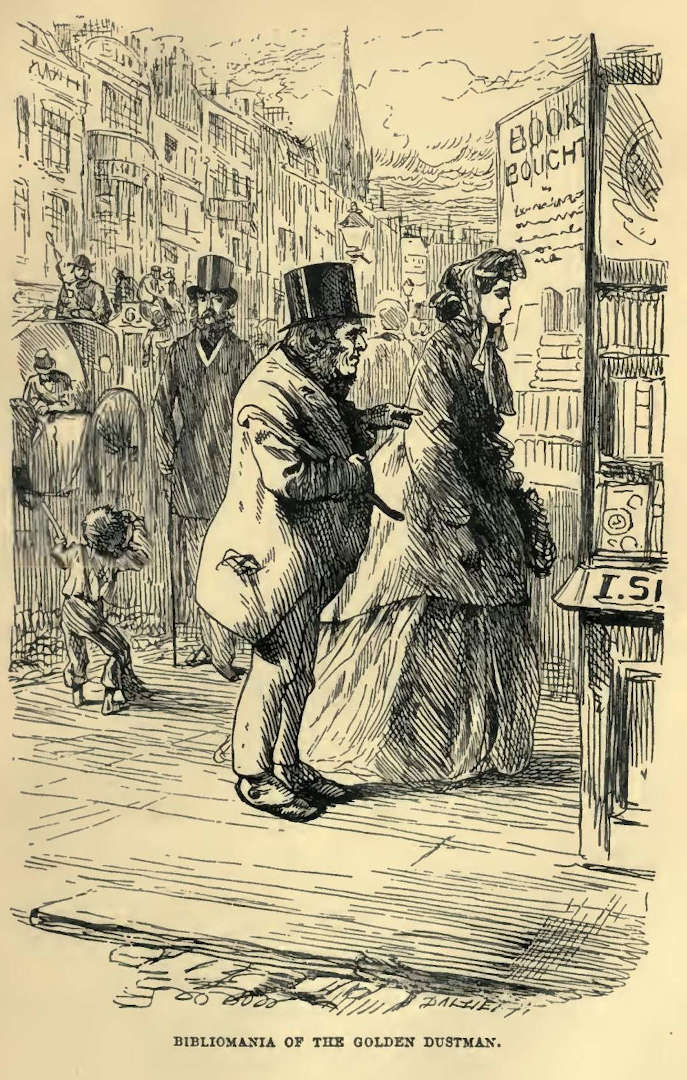
\includegraphics[scale=2.3]{03-05-01}

Chapter 10

THE DOLLS’ DRESSMAKER DISCOVERS A WORD


A darkened and hushed room; the river outside the windows flowing on
to the vast ocean; a figure on the bed, swathed and bandaged and bound,
lying helpless on its back, with its two useless arms in splints at its
sides. Only two days of usage so familiarized the little dressmaker
with this scene, that it held the place occupied two days ago by the
recollections of years.

He had scarcely moved since her arrival. Sometimes his eyes were open,
sometimes closed. When they were open, there was no meaning in their
unwinking stare at one spot straight before them, unless for a moment
the brow knitted into a faint expression of anger, or surprise. Then,
Mortimer Lightwood would speak to him, and on occasions he would be so
far roused as to make an attempt to pronounce his friend’s name. But, in
an instant consciousness was gone again, and no spirit of Eugene was in
Eugene’s crushed outer form.

They provided Jenny with materials for plying her work, and she had a
little table placed at the foot of his bed. Sitting there, with her rich
shower of hair falling over the chair-back, they hoped she might attract
his notice. With the same object, she would sing, just above her breath,
when he opened his eyes, or she saw his brow knit into that faint
expression, so evanescent that it was like a shape made in water. But
as yet he had not heeded. The ‘they’ here mentioned were the medical
attendant; Lizzie, who was there in all her intervals of rest; and
Lightwood, who never left him.

The two days became three, and the three days became four. At length,
quite unexpectedly, he said something in a whisper.

‘What was it, my dear Eugene?’

‘Will you, Mortimer--’

‘Will I--?

--‘Send for her?’

‘My dear fellow, she is here.’

Quite unconscious of the long blank, he supposed that they were still
speaking together.

The little dressmaker stood up at the foot of the bed, humming her song,
and nodded to him brightly. ‘I can’t shake hands, Jenny,’ said Eugene,
with something of his old look; ‘but I am very glad to see you.’

Mortimer repeated this to her, for it could only be made out by bending
over him and closely watching his attempts to say it. In a little while,
he added:

‘Ask her if she has seen the children.’

Mortimer could not understand this, neither could Jenny herself, until
he added:

‘Ask her if she has smelt the flowers.’

‘Oh! I know!’ cried Jenny. ‘I understand him now!’ Then, Lightwood
yielded his place to her quick approach, and she said, bending over the
bed, with that better look: ‘You mean my long bright slanting rows of
children, who used to bring me ease and rest? You mean the children who
used to take me up, and make me light?’

Eugene smiled, ‘Yes.’

‘I have not seen them since I saw you. I never see them now, but I am
hardly ever in pain now.’

‘It was a pretty fancy,’ said Eugene.

‘But I have heard my birds sing,’ cried the little creature, ‘and I have
smelt my flowers. Yes, indeed I have! And both were most beautiful and
most Divine!’

‘Stay and help to nurse me,’ said Eugene, quietly. ‘I should like you to
have the fancy here, before I die.’

She touched his lips with her hand, and shaded her eyes with that same
hand as she went back to her work and her little low song. He heard the
song with evident pleasure, until she allowed it gradually to sink away
into silence.

‘Mortimer.’

‘My dear Eugene.’

‘If you can give me anything to keep me here for only a few minutes--’

‘To keep you here, Eugene?’

‘To prevent my wandering away I don’t know where--for I begin to be
sensible that I have just come back, and that I shall lose myself
again--do so, dear boy!’

Mortimer gave him such stimulants as could be given him with safety
(they were always at hand, ready), and bending over him once more, was
about to caution him, when he said:

‘Don’t tell me not to speak, for I must speak. If you knew the
harassing anxiety that gnaws and wears me when I am wandering in those
places--where are those endless places, Mortimer? They must be at an
immense distance!’

He saw in his friend’s face that he was losing himself; for he added
after a moment: ‘Don’t be afraid--I am not gone yet. What was it?’

‘You wanted to tell me something, Eugene. My poor dear fellow, you
wanted to say something to your old friend--to the friend who has always
loved you, admired you, imitated you, founded himself upon you, been
nothing without you, and who, God knows, would be here in your place if
he could!’

‘Tut, tut!’ said Eugene with a tender glance as the other put his hand
before his face. ‘I am not worth it. I acknowledge that I like it,
dear boy, but I am not worth it. This attack, my dear Mortimer; this
murder--’

His friend leaned over him with renewed attention, saying: ‘You and I
suspect some one.’

‘More than suspect. But, Mortimer, while I lie here, and when I lie
here no longer, I trust to you that the perpetrator is never brought to
justice.’

‘Eugene?’

‘Her innocent reputation would be ruined, my friend. She would be
punished, not he. I have wronged her enough in fact; I have wronged her
still more in intention. You recollect what pavement is said to be made
of good intentions. It is made of bad intentions too. Mortimer, I am
lying on it, and I know!’

‘Be comforted, my dear Eugene.’

‘I will, when you have promised me. Dear Mortimer, the man must never be
pursued. If he should be accused, you must keep him silent and save
him. Don’t think of avenging me; think only of hushing the story
and protecting her. You can confuse the case, and turn aside the
circumstances. Listen to what I say to you. It was not the schoolmaster,
Bradley Headstone. Do you hear me? Twice; it was not the schoolmaster,
Bradley Headstone. Do you hear me? Three times; it was not the
schoolmaster, Bradley Headstone.’

He stopped, exhausted. His speech had been whispered, broken, and
indistinct; but by a great effort he had made it plain enough to be
unmistakeable.

‘Dear fellow, I am wandering away. Stay me for another moment, if you
can.’

Lightwood lifted his head at the neck, and put a wine-glass to his lips.
He rallied.

‘I don’t know how long ago it was done, whether weeks, days, or hours.
No matter. There is inquiry on foot, and pursuit. Say! Is there not?’

‘Yes.’

‘Check it; divert it! Don’t let her be brought in question. Shield
her. The guilty man, brought to justice, would poison her name. Let the
guilty man go unpunished. Lizzie and my reparation before all! Promise
me!’

‘Eugene, I do. I promise you!’

In the act of turning his eyes gratefully towards his friend, he
wandered away. His eyes stood still, and settled into that former intent
unmeaning stare.

Hours and hours, days and nights, he remained in this same condition.
There were times when he would calmly speak to his friend after a long
period of unconsciousness, and would say he was better, and would ask
for something. Before it could be given him, he would be gone again.

The dolls’ dressmaker, all softened compassion now, watched him with an
earnestness that never relaxed. She would regularly change the ice, or
the cooling spirit, on his head, and would keep her ear at the pillow
betweenwhiles, listening for any faint words that fell from him in his
wanderings. It was amazing through how many hours at a time she would
remain beside him, in a crouching attitude, attentive to his slightest
moan. As he could not move a hand, he could make no sign of distress;
but, through this close watching (if through no secret sympathy or
power) the little creature attained an understanding of him that
Lightwood did not possess. Mortimer would often turn to her, as if she
were an interpreter between this sentient world and the insensible man;
and she would change the dressing of a wound, or ease a ligature, or
turn his face, or alter the pressure of the bedclothes on him, with an
absolute certainty of doing right. The natural lightness and delicacy of
touch which had become very refined by practice in her miniature work,
no doubt was involved in this; but her perception was at least as fine.

The one word, Lizzie, he muttered millions of times. In a certain phase
of his distressful state, which was the worst to those who tended him,
he would roll his head upon the pillow, incessantly repeating the name
in a hurried and impatient manner, with the misery of a disturbed mind,
and the monotony of a machine. Equally, when he lay still and staring,
he would repeat it for hours without cessation, but then, always in a
tone of subdued warning and horror. Her presence and her touch upon his
breast or face would often stop this, and then they learned to expect
that he would for some time remain still, with his eyes closed, and that
he would be conscious on opening them. But, the heavy disappointment of
their hope--revived by the welcome silence of the room--was, that his
spirit would glide away again and be lost, in the moment of their joy
that it was there.

This frequent rising of a drowning man from the deep, to sink again, was
dreadful to the beholders. But, gradually the change stole upon him that
it became dreadful to himself. His desire to impart something that was
on his mind, his unspeakable yearning to have speech with his friend
and make a communication to him, so troubled him when he recovered
consciousness, that its term was thereby shortened. As the man rising
from the deep would disappear the sooner for fighting with the water, so
he in his desperate struggle went down again.

One afternoon when he had been lying still, and Lizzie, unrecognized,
had just stolen out of the room to pursue her occupation, he uttered
Lightwood’s name.

‘My dear Eugene, I am here.’

‘How long is this to last, Mortimer?’

Lightwood shook his head. ‘Still, Eugene, you are no worse than you
were.’

‘But I know there’s no hope. Yet I pray it may last long enough for you
to do me one last service, and for me to do one last action. Keep me
here a few moments, Mortimer. Try, try!’

His friend gave him what aid he could, and encouraged him to believe
that he was more composed, though even then his eyes were losing the
expression they so rarely recovered.

‘Hold me here, dear fellow, if you can. Stop my wandering away. I am
going!’

‘Not yet, not yet. Tell me, dear Eugene, what is it I shall do?’

‘Keep me here for only a single minute. I am going away again. Don’t let
me go. Hear me speak first. Stop me--stop me!’

‘My poor Eugene, try to be calm.’

‘I do try. I try so hard. If you only knew how hard! Don’t let me wander
till I have spoken. Give me a little more wine.’

Lightwood complied. Eugene, with a most pathetic struggle against the
unconsciousness that was coming over him, and with a look of appeal that
affected his friend profoundly, said:

‘You can leave me with Jenny, while you speak to her and tell her what I
beseech of her. You can leave me with Jenny, while you are gone. There’s
not much for you to do. You won’t be long away.’

‘No, no, no. But tell me what it is that I shall do, Eugene!’

‘I am going! You can’t hold me.’

‘Tell me in a word, Eugene!’

His eyes were fixed again, and the only word that came from his lips was
the word millions of times repeated. Lizzie, Lizzie, Lizzie.

But, the watchful little dressmaker had been vigilant as ever in her
watch, and she now came up and touched Lightwood’s arm as he looked down
at his friend, despairingly.

‘Hush!’ she said, with her finger on her lips. ‘His eyes are closing.
He’ll be conscious when he next opens them. Shall I give you a leading
word to say to him?’

‘O Jenny, if you could only give me the right word!’

‘I can. Stoop down.’

He stooped, and she whispered in his ear. She whispered in his ear one
short word of a single syllable. Lightwood started, and looked at her.

‘Try it,’ said the little creature, with an excited and exultant face.
She then bent over the unconscious man, and, for the first time, kissed
him on the cheek, and kissed the poor maimed hand that was nearest to
her. Then, she withdrew to the foot of the bed.

Some two hours afterwards, Mortimer Lightwood saw his consciousness come
back, and instantly, but very tranquilly, bent over him.

‘Don’t speak, Eugene. Do no more than look at me, and listen to me. You
follow what I say.’

He moved his head in assent.

‘I am going on from the point where we broke off. Is the word we should
soon have come to--is it--Wife?’

‘O God bless you, Mortimer!’

‘Hush! Don’t be agitated. Don’t speak. Hear me, dear Eugene. Your mind
will be more at peace, lying here, if you make Lizzie your wife. You
wish me to speak to her, and tell her so, and entreat her to be your
wife. You ask her to kneel at this bedside and be married to you, that
your reparation may be complete. Is that so?’

‘Yes. God bless you! Yes.’

‘It shall be done, Eugene. Trust it to me. I shall have to go away
for some few hours, to give effect to your wishes. You see this is
unavoidable?’

‘Dear friend, I said so.’

‘True. But I had not the clue then. How do you think I got it?’

Glancing wistfully around, Eugene saw Miss Jenny at the foot of the bed,
looking at him with her elbows on the bed, and her head upon her hands.
There was a trace of his whimsical air upon him, as he tried to smile at
her.

‘Yes indeed,’ said Lightwood, ‘the discovery was hers. Observe my dear
Eugene; while I am away you will know that I have discharged my trust
with Lizzie, by finding her here, in my present place at your bedside,
to leave you no more. A final word before I go. This is the right course
of a true man, Eugene. And I solemnly believe, with all my soul, that if
Providence should mercifully restore you to us, you will be blessed with
a noble wife in the preserver of your life, whom you will dearly love.’

‘Amen. I am sure of that. But I shall not come through it, Mortimer.’

‘You will not be the less hopeful or less strong, for this, Eugene.’

‘No. Touch my face with yours, in case I should not hold out till you
come back. I love you, Mortimer. Don’t be uneasy for me while you are
gone. If my dear brave girl will take me, I feel persuaded that I shall
live long enough to be married, dear fellow.’

Miss Jenny gave up altogether on this parting taking place between the
friends, and sitting with her back towards the bed in the bower made by
her bright hair, wept heartily, though noiselessly. Mortimer Lightwood
was soon gone. As the evening light lengthened the heavy reflections of
the trees in the river, another figure came with a soft step into the
sick room.

‘Is he conscious?’ asked the little dressmaker, as the figure took its
station by the pillow. For, Jenny had given place to it immediately, and
could not see the sufferer’s face, in the dark room, from her new and
removed position.

‘He is conscious, Jenny,’ murmured Eugene for himself. ‘He knows his
wife.’



